\scanpage{76}
\[
f_\varphi(\rho)=\rho^p\int\frac{s^{-p}}{1+s}\,ds=c^{\mathrm{te}}.\rho^p,
\]

d'où, en posant \deleted{\unsure{Système|$S_p^{(n)}$}} a.

\[
S_p^{(n)}(u)=\sum_1^n\rho_i(u)^p
\]

\[
\boxed{S_p^{(n)}(u+v)\leq S_p^{(n)}(u)+S_p^{(n)}(v)}
\]

en particulier

\[
\boxed{S_p(u+v)\leq S_p(u)\unsure{-|+}S_p(v)}
\]

\reversemarginpar
\margin{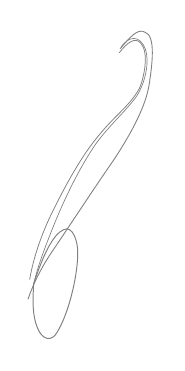
\begin{tikzpicture}[x=.1mm,y=-.1mm,line cap=round,line join=round,color=gray]
\draw[line width=.32pt] (138,33) .. controls (150,19) and (160,7) .. (169,12) .. controls (184,16) and (178,56) .. (175,77) .. controls (171,105) and (153,139) .. (130,174) .. controls (101,216) and (77,253) .. (52,290) .. controls (37,312) and (27,333) .. (21,351);
\draw[line width=.28pt] (137,38) .. controls (147,25) and (157,18) .. (164,26) .. controls (175,38) and (168,70) .. (163,82) .. controls (153,103) and (131,118) .. (111,143) .. controls (89,169) and (70,204) .. (53,238) .. controls (39,266) and (28,297) .. (23,326);
\draw[line width=.25pt] (139,31) .. controls (149,17) and (163,15) .. (170,34) .. controls (176,53) and (168,81) .. (157,96) .. controls (144,113) and (123,132) .. (107,154) .. controls (87,183) and (66,225) .. (49,269) .. controls (40,292) and (31,316) .. (27,337);
\draw[line width=.35pt] (28,332) .. controls (39,298) and (52,269) .. (66,263) .. controls (77,257) and (85,277) .. (84,296) .. controls (83,326) and (72,370) .. (58,393) .. controls (51,406) and (39,403) .. (33,388) .. controls (26,372) and (27,351) .. (28,332);
\end{tikzpicture}}
\normalmarginpar

\uline{Remarque} On a $\sum_1^n\rho_i(u+v)^p\leq\sum_1^n(\rho_i(u)^p+\rho_i(v)^p)$, quel que soit $n$, on peut donc appliquer le lemme de Weyl ; on trouve rien de spécial.

\uline{Question} Trouver la forme générale des fonctions $f$ d'une variable positive telle que, posant \deleted{\unsure{$S_f^{(n)}(u)$}} $f^{(n)}(u)=\sum_1^n\rho_i(u)$, on ait $f^{(n)}(u+v)\leq f^{(n)}(u)+f^{(n)}(v)$ quel que soit $n$. Il suffit qu'on ait $f^{\infty}(u+v)\leq f^{\infty}(u)+f^{\infty}(v)$

pour \uline{tout} $u\in L(E)$, avec $E$ espace de Hilbert de dimension finie arbitraire. Généralisation à des fonctions de $n$ arguments.

\figure{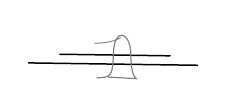
\begin{tikzpicture}[x=1mm,y=1mm,line cap=round]
\draw[line width=.19mm] (4,3)--(18,2.8) (0,1.9)--(21.5,1.6);
\draw[gray,line width=.15mm] (8.7,0).. controls (10.5,.1) and (10.7,.1)..(10.8,3.2)..controls (10.9,6.3) and (12.8,6)..(13,3.3)..controls (13,.8) and (13.4,.1)..(13.7,-.1)--(10.1,.1);
\draw[gray,line width=.12mm] (8.4,4.4)..controls (10.2,4.4) and (11.2,4.8)..(11.7,5.1);
\end{tikzpicture}}

\margin{77}
